%% poster.tex
%% Vorlage fr A0-Poster
%% Harry Schmidt
%% 25.04.2003

%% translation instructions (there should be a better way):
%% latex ...
%% dvips -Ppdf -D9600 ...
%% psresize -w84cm -h118.8cm ... outfile.ps
%% edit postscript to position and size poster correctly
%%    bounding box in ps: 0 0 2380 3368
%%    after %%EndComments add:  gsave 0 -140 translate
%%    before showpage     add:  grestore
%% (adjust voffset and hoffset below to center text on page)
%% ps2pdf -sPAPERSIZE=a0 poster2a.ps


\documentclass{theo1poster}[2003/04/25]
\textwidth=11in                 % real width of latex text 
\textheight=11in                % height of latex text
\special{papersize=11.7in,11.7in}   % small width ensures portrait orientation
\addtolength{\voffset}{-.7in}
\addtolength{\textheight}{1.5cm}
\addtolength{\voffset}{52pt}  %% depends on actual length of poster
\addtolength{\hoffset}{8pt}   %% probably universal
%\usepackage[american,ngerman]{babel}
\usepackage[latin1]{inputenc}
\usepackage[T1]{fontenc}
%\usepackage{ae}
\usepackage{amsmath,amssymb,psfrag,pifont}
\usepackage{graphicx}

%% Farben

\definecolor{lightblue}{rgb}{0.75,0.8,1}
\definecolor{graublau}{rgb}{0.85,0.85,0.9}
\definecolor{gruen}{rgb}{0.0,0.4,0.0}
\definecolor{alexblue}{rgb}{0.8,0.64,0.0}
\definecolor{strangeyellow}{rgb}{0.875,1.0,0.08}
\definecolor{verylightgray}{gray}{0.99}
\definecolor{meinrot}{rgb}{0.8,0.1,0.2}
\definecolor{lightocker}{rgb}{1,0.9,0.6}
\definecolor{orange}{rgb}{1,0.5,0}
\definecolor{darkorange}{rgb}{0.7,0.35,0}


\definecolor{sheetbg}{rgb}{0.75,0.8,1}
\definecolor{boxbg}{rgb}{1,1,0.95}
\definecolor{boxrahmen}{rgb}{0.11,0.15,0.4}


%% Stil-Befehle fr das Poster, kann fr jedes
%% einzelne Poster festgelegt werden

\posterbgcolor{sheetbg}    %% Hintergrundfarbe des Posters
%\posterbgcolor{lightocker}
%\posterbgcolor{lightblue}
%\posterbgcolor{graublau}


%\titlecolor{black}         %% Farbe des Titels
\headingcolor{black}       %% Farbe der �erschriften
%\headingcolor{meinrot}

%\headingfont{\sffamily}    %% Font der �erschriften
%\headingfontsize{\large}   %% Fontgr�e der �erschriften

\sheetframewidth{1mm}    %% Breite des Sheet-Rahmens
\sheetframesep{3pt}        %% Abstand des Textes vom Rahmen

\sheetframecolor{boxrahmen}    %% Farbe des Sheet-Rahmens
%\sheetframecolor{boxbg}
\sheetbgcolor{boxbg}       %% Farbe des Sheet-Hintergrunds
%\sheetbgcolor{verylightgray}

\colorsheets               %% Wird automatisch von \sheet..color  ausgefhrt
%\nocolorsheets             %% Default, solange \sheet..color nicht aufgerufen
%\roundsheets               %% Abgerundete Ecken ohne Farbe
\roundcolorsheets          %% Farbig und abgerundete Ecken

%\highlightcolor{lightocker} %% Farbe fr Hervorhebungen (Formeln)

%\renewcommand*\sectfont{\sffamily}
%\renewcommand*\sectfont{\bfseries\mathversion{bold}}

%\renewcommand*\bfdefault{b}


%% Sonstige Befehle

\renewcommand{\labelitemi}{\ding{228}}
\renewenvironment{itemize}% Liste mit bullet in gegebenem Abstand
                              % von linkem Rand der umschliessenden Umgebung
                              % M. Stollsteimer, 15.1.2001
 {\begin{list}{\labelitemi}%
       {%
%        \setlength{\topsep}{0pt}% Abstand vor Liste
        \setlength{\leftmargin}{0pt}% Raum vor bullet
        \setlength{\itemindent}{0pt}% Einrckung der ersten Zeile
        \settowidth{\labelwidth}{\labelitemi}%
        \addtolength{\labelsep}{\itemindent}
        \addtolength{\leftmargin}{\labelwidth}%
        \addtolength{\leftmargin}{\labelsep}%
        \addtolength{\leftmargin}{-\itemindent}%
       }%
 }
 {\end{list}}

\newenvironment{itemizenotopsep}{% Wie oben, nur mit \topsep=0pt
  \begin{list}{\labelitemi}%
    {%
      \setlength{\topsep}{0pt}% Abstand vor Liste
      \setlength{\leftmargin}{0pt}% Raum vor bullet
      \setlength{\itemindent}{0pt}% Einrckung der ersten Zeile
      \setlength{\itemsep}{0.5pt}% vertikaler Abstand von Items
      \setlength{\parsep}{1.5pt}%
      \settowidth{\labelwidth}{\labelitemi}%
      \addtolength{\labelsep}{\itemindent}
      \addtolength{\leftmargin}{\labelwidth}%
      \addtolength{\leftmargin}{\labelsep}%
      \addtolength{\leftmargin}{-\itemindent}}%
    }
  {\end{list}}


%% Daten fr den Titel

\title{Identification of multidimensional semiclassical tunneling paths}
\author{Predrag Cvitanovi\'c\ensuremath{^*}, Ruslan L. Davidchack\ensuremath{^\dagger} and Evangelos Siminos\ensuremath{^*}}
\newlength{\addresswidth}
 
\address{ \ensuremath{^*} Center for Nonlinear Science, Georgia Institute of Technology, 
          Atlanta, GA 30332-0430, USA\\
\ensuremath{^\dagger} Department of Mathematics, University of Leicester,
            University Road, Leicester LE1 7RH, UK
}


%\settowidth{\addresswidth}%
%       {\large Center for Nonlinear Science, Georgia Institute of Technology,}
%\address{\parbox{\addresswidth} {\centering%
%           Center for Nonlinear Science, Georgia Institute of Technology, 
%           Atlanta, GA 30332-0430, USA}%
%        }
%\logo{GT.eps}
%\setlength{\logowidth}{3cm}

%% Wem die Titelei nicht gef�lt:
%\renewcommand{\maketitle}{eigene Titelei}




\begin{document}


\begin{poster}{3}

\begin{sheet}{Introduction}
Many reaction rates in physics and chemistry are determined by quantum
mechanical tunneling below a classically insurmountable barrier.
In the semi-

\noindent
\begin{minipage}[c]{.49\textwidth}
classical approximation, the tunneling transmission probability is
determined by the action integral
\begin{equation}
%  \label{TunnAct}
  K=\int |p|\,dq
\end{equation}
along the tunneling path. The latter is easy to identify in one-dimensional
problems as the straight line path below\, the barrier,\, but\, in systems
\hfill with
\end{minipage}
\begin{minipage}[c]{.47\textwidth}
\centerline{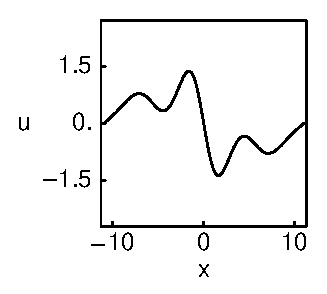
\includegraphics[width=.95\textwidth]{../../figs/1wKS22equil.eps}}
\end{minipage}
\noindent
several degrees of freedom it can deviate markedly from being straight.
As a further complication, oscillations transverse to the reaction
coordinate can be excited in multidimensional systems.

If reactant and product regions of configuration space are separated by a
saddle point in a multidimensional potential, the path of steepest descent
from the saddle is regarded as the ``reaction path'' in chemistry (see, eg.,
\cite{Truhlar96}). However, it is also well known that the tunneling
integral taken along that path severely underestimates the tunneling
probability. The true tunneling path tends to lie on the concave
side of the reaction path (``corner cutting''). In the absence of
transverse excitation, it can be identified as the configuration space
projection of an imaginary-time complex periodic orbit. How best to include
the effects of the transverse modes is still a hotly debated topic in
reaction rate theory.

I will here demonstrate that normal form theory allows a decoupling of the
degrees of freedom and permits an identification
of the tunneling path in the absence and in the presence of transverse
excitation.
\end{sheet}


\begin{sheet}{Tunneling in multiple degrees of freedom}
We assume that the saddle point is unstable in one degree of freedom, which
is the reaction coordinate, and stable in all others.
The optimal tunneling path is easy to identify if the
different degrees of freedom decouple, as in the Hamiltonian
\begin{equation}
  H=\frac{\lambda}{2}(p_x^2-x^2) + \frac{\omega_y}{2}(p_y^2+y^2)
   +\frac{\omega_z}{2}(p_z^2+z^2) \;.
\end{equation}
Here $x$ represents the reaction coordinate and $y$ and $z$ are transverse
coordinates. In this case, the optimum tunneling path can be found by
setting the transverse coordinates to their equilibrium values
$y=p_y=z=p_z=0$, which reduces the problem to one degree of freedom. The
tunneling integral can then be computed from the reduced problem in the
usual way.

In general, a multidimensional dynamical system is non-separable. However,
if its Hamiltonian is expanded in a multidimensional power series around an
equilibrium point, normal form theory (see, eg., \cite{Jorba99}) allows one
to construct a coordinate transformation that puts the Hamiltonian into a
separable form up to an arbitrarily high finite order.  The high-order
remainder that has not been brought into normal form is then neglected.
\end{sheet}


\begin{sheet}{Tunneling paths}
Once the tunneling path has been determined in normal form coordinates, it
can be transformed to laboratory coordinates. The tunneling path thus
found coincides with the projection of the periodic tunneling orbit into the
configuration space.

This is here illustrated for the dynamics of an electron under the combined
influences of two identical Coulomb centers and a homogeneous electric
field. This system has been used as a simple model for the ionization of a
$H_2^+$ molecular ion by a laser field \cite{Bandrauk00}. In the example
shown, the Coulomb centers are located at $x=z=0, y=\pm 1\,\text{a.u.}$ The
external field strength is $0.77\,\text{a.u.}$, and the field makes an
angle of 84.3 degrees with the molecular axis. For these parameter
values the reaction path is highly curved.

\centerline{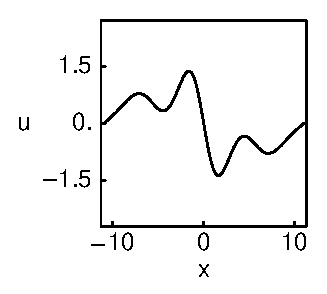
\includegraphics[width=.85\textwidth]{../../figs/1wKS22equil.eps}}
\end{sheet}



\begin{sheet}{Tunneling action}
Freezing the transverse degrees of freedom to equilibrium reduces the
normal form Hamiltonian to a one-dimensional tunneling Hamiltonian
given as a power series in the tunneling action. This series can be
inverted to obtain the action as a function of energy.

In practice, the power series for the action
converges only very close to the saddle. By means of a Pad\'e transform,
however, useful values for the tunneling action can still be computed
even far below the saddle point energy. It can then be observed how with
increasing order the normal-form result converges to the action of the
periodic tunneling orbit, whereas the action along the steepest-descent
``reaction path'' is markedly larger and thus significantly underestimates
the tunneling probability.

\centerline{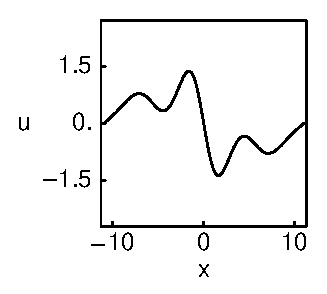
\includegraphics[width=.96\textwidth]{../../figs/1wKS22equil.eps}}
\end{sheet}


\begin{sheet}{Transverse frequencies}
In a similar manner, the frequencies of the transverse normal modes can be
computed from the terms in the normal form Hamiltonian that are quadratic
in the transverse coordinates.

In the figure, solid lines denote frequencies of the linearized motion
around the periodic tunneling orbit. Dashed lines indicate frequencies
obtained from a normal form calculation of order 4, 8, 12 or 16, respectively.

\centerline{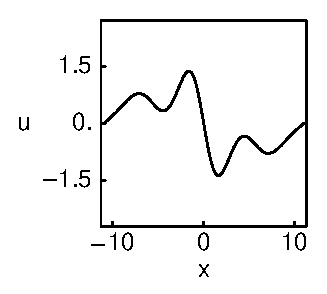
\includegraphics[width=.96\textwidth]{../../figs/1wKS22equil.eps}}
\end{sheet}



\begin{sheet}{Effects of transverse modes}
The optimal tunneling paths described above were calculated under the
assumption that there is no excitation of the transverse degrees of
freedom. In practice, however, the transverse modes will always be excited
at least to their zero-point oscillations. The normal form approach to
tunneling lends itself easily to an inclusion of transverse vibrations: It
allows to construct a complete set of action coordinates that are conserved
under the truncated dynamics. They can be set to arbitrary non-zero values
if the corresponding nonlinear normal modes are excited. Then, as before,
the normal form yields the energy as a power series in the tunneling
action, which can be inverted to obtain the action as a function of energy.

\end{sheet}


\begin{sheet}{References}
\begin{thebibliography}{5}
\bibitem{Truhlar96}
  D.~G.~Truhlar, B.~C.~Garrett, and S.~J.~Klippenstein:
  \emph{J.~Phys.~Chem.} \textbf{100} (1996), 12771--12800
\bibitem{Jorba99}
  \`A.~Jorba: \emph{Exp.~Math.} \textbf{8} (1999), 155--195
\bibitem{Bandrauk00}
  A.~D.~Bandrauk and H. Z. Lu: \emph{Phys.~Rev.~A} \textbf{62} (2000), 053406
\end{thebibliography}
\end{sheet}



\end{poster}


\end{document}
